
\documentclass[letterpaper,hide notes,xcolor={table,svgnames},pdftex,10pt]{beamer}
\def\showexamples{t}


%\usepackage[svgnames]{xcolor}

%% Demo talk
%\documentclass[letterpaper,notes=show]{beamer}

\usecolortheme{crane}
\setbeamertemplate{navigation symbols}{}

\usetheme{MyPittsburgh}
%\usetheme{Frankfurt}

%\usepackage{tipa}

\usepackage{hyperref}
\usepackage{graphicx,xspace}
\usepackage[normalem]{ulem}
\usepackage{multicol}
\usepackage{amsmath,amssymb,amsthm,graphicx,xspace}
\newcommand\SF[1]{$\bigstar$\footnote{SF: #1}}

\usepackage[default]{sourcesanspro}
\usepackage[T1]{fontenc}

\newcounter{tmpnumSlide}
\newcounter{tmpnumNote}

% old question code
%\newcommand\question[1]{{$\bigstar$ \small \onlySlide{2}{#1}}}
% \newcommand\nquestion[1]{\ifdefined \presentationonly \textcircled{?} \fi \note{\par{\Large \textbf{?}} #1}}
% \newcommand\nanswer[1]{\note{\par{\Large \textbf{A}} #1}}


 \newcommand\mnote[1]{%
   \addtocounter{tmpnumSlide}{1}
   \ifdefined\showcues {~\tiny\fbox{\arabic{tmpnumSlide}}}\fi
   \note{\setlength{\parskip}{1ex}\addtocounter{tmpnumNote}{1}\textbf{\Large \arabic{tmpnumNote}:} {#1\par}}}

\newcommand\mmnote[1]{\note{\setlength{\parskip}{1ex}#1\par}}

%\newcommand\mnote[2][]{\ifdefined\handoutwithnotes {~\tiny\fbox{#1}}\fi
% \note{\setlength{\parskip}{1ex}\textbf{\Large #1:} #2\par}}

%\newcommand\mnote[2][]{{\tiny\fbox{#1}} \note{\setlength{\parskip}{1ex}\textbf{\Large #1:} #2\par}}

\newcommand\mquestion[2]{{~\color{red}\fbox{?}}\note{\setlength{\parskip}{1ex}\par{\Large \textbf{?}} #1} \note{\setlength{\parskip}{1ex}\par{\Large \textbf{A}} #2\par}\ifdefined \presentationonly \pause \fi}

\newcommand\blackboard[1]{%
\ifdefined   \showblackboard
  {#1}
  \else {\begin{center} \fbox{\colorbox{blue!30}{%
         \begin{minipage}{.95\linewidth}%
           \hspace{\stretch{1}} Some space intentionally left blank; done at the blackboard.%
         \end{minipage}}}\end{center}}%
         \fi%
}



%\newcommand\q{\tikz \node[thick,color=black,shape=circle]{?};}
%\newcommand\q{\ifdefined \presentationonly \textcircled{?} \fi}

\usepackage{listings}
\lstset{%
  keywordstyle=\bfseries,
  aboveskip=15pt,
  belowskip=15pt,
  captionpos=b,
  identifierstyle=\ttfamily,
  escapeinside={(*@}{@*)},
  stringstyle=\ttfamiliy,
  frame=lines,
  numbers=left, basicstyle=\scriptsize, numberstyle=\tiny, stepnumber=0, numbersep=2pt}

\usepackage{siunitx}
\newcommand\sius[1]{\num[group-separator = {,}]{#1}\si{\micro\second}}
\newcommand\sims[1]{\num[group-separator = {,}]{#1}\si{\milli\second}}
\newcommand\sins[1]{\num[group-separator = {,}]{#1}\si{\nano\second}}
\sisetup{group-separator = {,}, group-digits = true}

%% -------------------- tikz --------------------
\usepackage{tikz}
\usetikzlibrary{positioning}
\usetikzlibrary{arrows,backgrounds,automata,decorations.shapes,decorations.pathmorphing,decorations.markings,decorations.text}

\tikzstyle{place}=[circle,draw=blue!50,fill=blue!20,thick, inner sep=0pt,minimum size=6mm]
\tikzstyle{transition}=[rectangle,draw=black!50,fill=black!20,thick, inner sep=0pt,minimum size=4mm]

\tikzstyle{block}=[rectangle,draw=black, thick, inner sep=5pt]
\tikzstyle{bullet}=[circle,draw=black, fill=black, thin, inner sep=2pt]

\tikzstyle{pre}=[<-,shorten <=1pt,>=stealth',semithick]
\tikzstyle{post}=[->,shorten >=1pt,>=stealth',semithick]
\tikzstyle{bi}=[<->,shorten >=1pt,shorten <=1pt, >=stealth',semithick]

\tikzstyle{mut}=[-,>=stealth',semithick]

\tikzstyle{treereset}=[dashed,->, shorten >=1pt,>=stealth',thin]

\usepackage{ifmtarg}
\usepackage{xifthen}
\makeatletter
% new counter to now which frame it is within the sequence
\newcounter{multiframecounter}
% initialize buffer for previously used frame title
\gdef\lastframetitle{\textit{undefined}}
% new environment for a multi-frame
\newenvironment{multiframe}[1][]{%
\ifthenelse{\isempty{#1}}{%
% if no frame title was set via optional parameter,
% only increase sequence counter by 1
\addtocounter{multiframecounter}{1}%
}{%
% new frame title has been provided, thus
% reset sequence counter to 1 and buffer frame title for later use
\setcounter{multiframecounter}{1}%
\gdef\lastframetitle{#1}%
}%
% start conventional frame environment and
% automatically set frame title followed by sequence counter
\begin{frame}%
\frametitle{\lastframetitle~{\normalfont(\arabic{multiframecounter})}}%
}{%
\end{frame}%
}
\makeatother

\makeatletter
\newdimen\tu@tmpa%
\newdimen\ydiffl%
\newdimen\xdiffl%
\newcommand\ydiff[2]{%
    \coordinate (tmpnamea) at (#1);%
    \coordinate (tmpnameb) at (#2);%
    \pgfextracty{\tu@tmpa}{\pgfpointanchor{tmpnamea}{center}}%
    \pgfextracty{\ydiffl}{\pgfpointanchor{tmpnameb}{center}}%
    \advance\ydiffl by -\tu@tmpa%
}
\newcommand\xdiff[2]{%
    \coordinate (tmpnamea) at (#1);%
    \coordinate (tmpnameb) at (#2);%
    \pgfextractx{\tu@tmpa}{\pgfpointanchor{tmpnamea}{center}}%
    \pgfextractx{\xdiffl}{\pgfpointanchor{tmpnameb}{center}}%
    \advance\xdiffl by -\tu@tmpa%
}
\makeatother
\newcommand{\copyrightbox}[3][r]{%
\begin{tikzpicture}%
\node[inner sep=0pt,minimum size=2em](ciimage){#2};
\usefont{OT1}{phv}{n}{n}\fontsize{4}{4}\selectfont
\ydiff{ciimage.south}{ciimage.north}
\xdiff{ciimage.west}{ciimage.east}
\ifthenelse{\equal{#1}{r}}{%
\node[inner sep=0pt,right=1ex of ciimage.south east,anchor=north west,rotate=90]%
{\raggedleft\color{black!50}\parbox{\the\ydiffl}{\raggedright{}#3}};%
}{%
\ifthenelse{\equal{#1}{l}}{%
\node[inner sep=0pt,right=1ex of ciimage.south west,anchor=south west,rotate=90]%
{\raggedleft\color{black!50}\parbox{\the\ydiffl}{\raggedright{}#3}};%
}{%
\node[inner sep=0pt,below=1ex of ciimage.south west,anchor=north west]%
{\raggedleft\color{black!50}\parbox{\the\xdiffl}{\raggedright{}#3}};%
}
}
\end{tikzpicture}
}


%% --------------------

%\usepackage[excludeor]{everyhook}
%\PushPreHook{par}{\setbox0=\lastbox\llap{MUH}}\box0}

%\vspace*{\stretch{1}

%\setbox0=\lastbox \llap{\textbullet\enskip}\box0}

\setlength{\parskip}{\fill}

\newcommand\noskips{\setlength{\parskip}{1ex}}
\newcommand\doskips{\setlength{\parskip}{\fill}}

\newcommand\xx{\par\vspace*{\stretch{1}}\par}
\newcommand\xxs{\par\vspace*{2ex}\par}
\newcommand\tuple[1]{\langle #1 \rangle}
\newcommand\code[1]{{\sf \footnotesize #1}}
\newcommand\ex[1]{\uline{Example:} \ifdefined \presentationonly \pause \fi
  \ifdefined\showexamples#1\xspace\else{\uline{\hspace*{2cm}}}\fi}

\newcommand\ceil[1]{\lceil #1 \rceil}


\AtBeginSection[]
{
   \begin{frame}
       \frametitle{Outline}
       \tableofcontents[currentsection]
   \end{frame}
}



\pgfdeclarelayer{edgelayer}
\pgfdeclarelayer{nodelayer}
\pgfsetlayers{edgelayer,nodelayer,main}

\tikzstyle{none}=[inner sep=0pt]
\tikzstyle{rn}=[circle,fill=Red,draw=Black,line width=0.8 pt]
\tikzstyle{gn}=[circle,fill=Lime,draw=Black,line width=0.8 pt]
\tikzstyle{yn}=[circle,fill=Yellow,draw=Black,line width=0.8 pt]
\tikzstyle{empty}=[circle,fill=White,draw=Black]
\tikzstyle{bw} = [rectangle, draw, fill=blue!20, 
    text width=4em, text centered, rounded corners, minimum height=2em]
    
    \newcommand{\CcNote}[1]{% longname
	This work is licensed under the \textit{Creative Commons #1 3.0 License}.%
}
\newcommand{\CcImageBy}[1]{%
	\includegraphics[scale=#1]{creative_commons/cc_by_30.pdf}%
}
\newcommand{\CcImageSa}[1]{%
	\includegraphics[scale=#1]{creative_commons/cc_sa_30.pdf}%
}
\newcommand{\CcImageNc}[1]{%
	\includegraphics[scale=#1]{creative_commons/cc_nc_30.pdf}%
}
\newcommand{\CcGroupBySa}[2]{% zoom, gap
	\CcImageBy{#1}\hspace*{#2}\CcImageNc{#1}\hspace*{#2}\CcImageSa{#1}%
}
\newcommand{\CcLongnameByNcSa}{Attribution-NonCommercial-ShareAlike}

\newenvironment{changemargin}[1]{% 
  \begin{list}{}{% 
    \setlength{\topsep}{0pt}% 
    \setlength{\leftmargin}{#1}% 
    \setlength{\rightmargin}{1em}
    \setlength{\listparindent}{\parindent}% 
    \setlength{\itemindent}{\parindent}% 
    \setlength{\parsep}{\parskip}% 
  }% 
  \item[]}{\end{list}} 




\def\ojoin{\setbox0=\hbox{$\bowtie$}%
  \rule[-.02ex]{.25em}{.4pt}\llap{\rule[\ht0]{.25em}{.4pt}}}
\def\leftouterjoin{\mathbin{\ojoin\mkern-5.8mu\bowtie}}

\title{Tutorial 7 --- Data Mining and Transactions }

\author{Richard Wong \\ \small \texttt{rk2wong@edu.uwaterloo.ca}}
\institute{Department of Electrical and Computer Engineering \\
  University of Waterloo}
\date{\today}


\begin{document}

\begin{frame}
  \titlepage

\end{frame}


\begin{frame}
\frametitle{Exercise 7-1}

What is a data warehouse, and why is it useful to have one?

\end{frame}


\begin{frame}
\frametitle{Exercise 7-1 Solution}

What is a data warehouse, and why is it useful to have one?

\begin{itemize}
  \item Maintain OLTP responsiveness by having separate hardware handle OLAP queries
  \item A data warehouse can be optimized for read access
  \item Reshape (denormalize) OLTP schema into star/snowflake schema to simplify OLAP queries
  \item Star/snowflake schemas enable cubing operations on data (look up "OLAP cube")
  \item Most OLAP queries deal in aggregates, which could benefit from column-oriented storage
  \item and more...
\end{itemize}

\end{frame}


\begin{frame}
\frametitle{Exercise 7-2}

Suppose we are trying to predict the value \textit{Wait}. \\
Between attributes \textit{Pat} and \textit{Type}, which is better to split a decision node on?

\begin{center}
  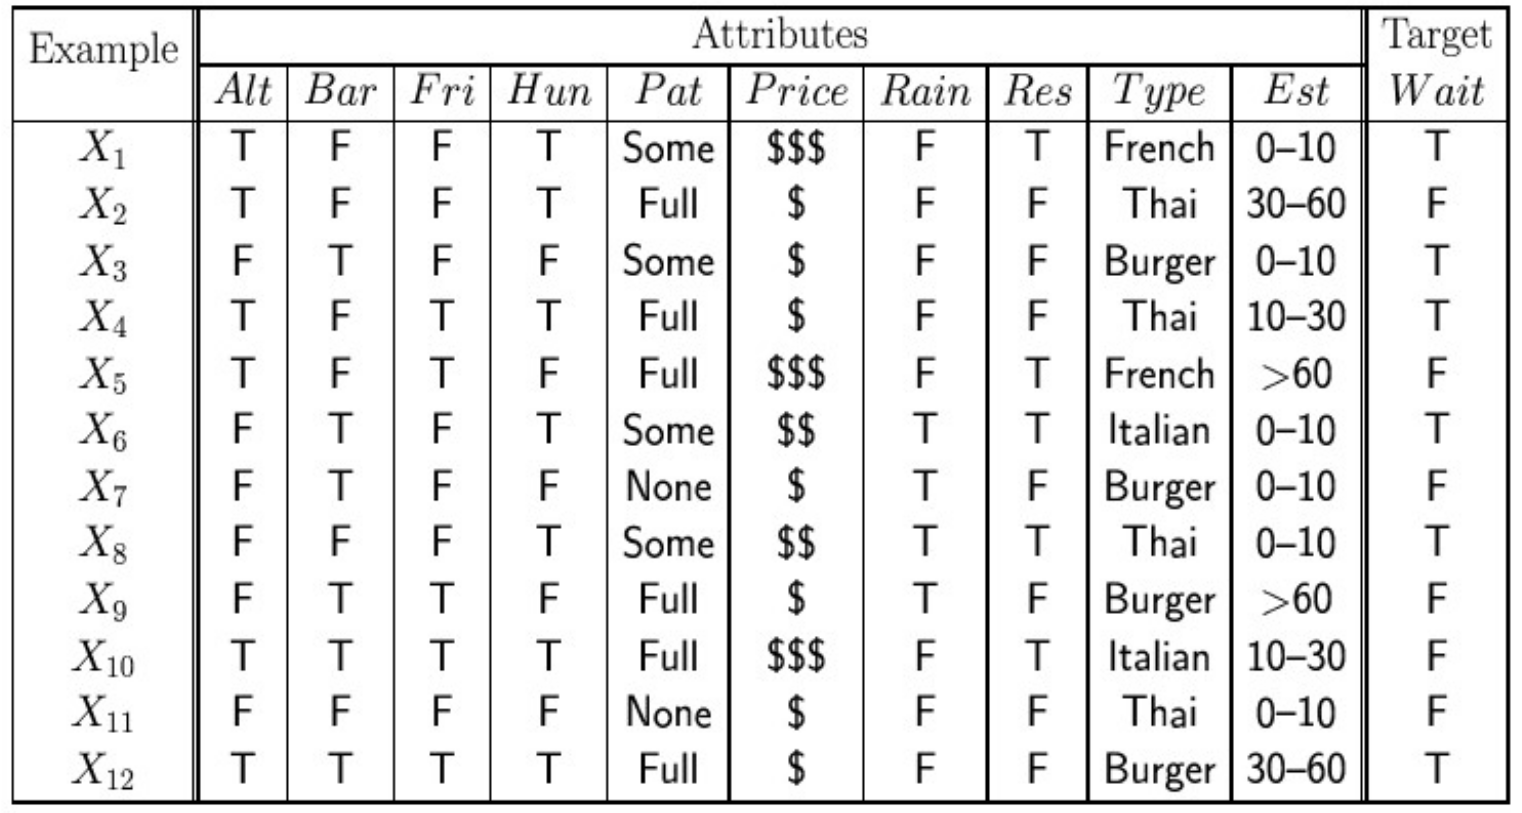
\includegraphics[width=0.9\textwidth]{images/decision_matrix.png}
\end{center}

\end{frame}


\begin{frame}
\frametitle{Exercise 7-2 Solution (1/3)}

Let's use entropy ($I$) as the metric that we want to minimize.

We have two choices of attributes (\textit{Pat} and \textit{Type}), and we want to pick the one that maximizes information gain. So first we should find out the entropy of the full data set $S$.

\begin{align*}
  I(S) &= -\sum_{i=1}^{\{T, F\}}p_i\log_2(p_i) \\
  &= -p_T\log_2(p_T) - p_F\log_2(p_F) \\
  &= -(\frac{6}{12})\log_2(\frac{6}{12}) - (\frac{6}{12})\log_2(\frac{6}{12}) \\
  &= -(\frac{1}{2})(-1) - (\frac{1}{2})(-1) \\
  &= \frac{1}{2} + \frac{1}{2} \\
  &= 1
\end{align*}

\end{frame}


\begin{frame}
\frametitle{Exercise 7-2 Solution (2/3)}

So $I(S) = 1$.

\begin{align*}
  I(S_{Pat}) &= P_{Pat=None}I(S_{Pat=None}) + P_{Pat=Some}I(S_{Pat=Some}) + P_{Pat=Full}I(S_{Pat=Full}) \\
  &= \frac{2}{12}(0) + \frac{4}{12}(0) + \frac{6}{12}I(S_{Pat=Full}) \\
  &= \frac{1}{2} (0.918) \\
  IG_{Pat} &= I(S) - I(S_{Pat}) \\
  &= 1 - \frac{1}{2} (0.918) \\
  &= 0.541
\end{align*}

\end{frame}


\begin{frame}
\frametitle{Exercise 7-2 Solution (3/3)}

\begin{align*}
  I(S_{Type}) &= P_{Type=French}I(S_{Type=French}) + P_{Type=Italian}I(S_{Type=Italian}) \\
  &+ P_{Type=Thai}I(S_{Type=Thai}) + P_{Type=Burger}I(S_{Type=Burger}) \\
  &= \frac{1}{4}(1) + \frac{1}{4}(1) + \frac{1}{4}(1) + \frac{1}{4}(1) \\
  &= 1 \\
  IG(S_{Type}) &= I(S) - I(S_{Type}) \\
  &= 1 - 1 \\
  &= 0
\end{align*}

So $IG(S_{Pat}) = 0.541$, $IG(S_{Type}) = 0$. \\
$IG(S_{Pat}) > IG(S_{Type})$, so $Pat$ is the better attribute to split on.

\end{frame}


\begin{frame}
\frametitle{Exercise 7-3}

What are the ACID transaction properties, and what can a database do to ensure each one?

\end{frame}


\begin{frame}
\frametitle{Exercise 7-3 Solution (1/2)}

The ACID properties:

\begin{itemize}
  \item Atomicity: the effects of a transaction either fully take place, or none at all.
  \item Consistency preservation: the state of a database before and after a transaction is consistent.
  \item Isolation: transactions can operate unaware of concurrent transactions.
  \item Durability: transaction completion guarantees persistence (i.e. write to disk or stable storage, backup, etc.)
\end{itemize}

\end{frame}


\begin{frame}
\frametitle{Exercise 7-3 Solution (2/2)}

How do we ensure each one?

\begin{itemize}
  \item Atomicity: keep a sequential log of each task that executes in a transaction. Each log entry should contain sufficient data to roll back. In addition, only allow execution of recoverable transaction schedules.
  \item Consistency: abort transactions that would violate constraints.
  \item Isolation: this can be done to varying degrees. It is up to the transaction manager to uphold isolation guarantees, which the DBA may decide on.
  \item Durability: never report that a transaction is committed until it is persisted.
\end{itemize}

\end{frame}


\begin{frame}
\frametitle{Exercise 7-4}

Distinguish between the following:

\begin{enumerate}
  \item a serial schedule
  \item a serializable schedule
  \item a conflict-serializable schedule
\end{enumerate}

\end{frame}


\begin{frame}
\frametitle{Exercise 7-4 Solution}

\begin{enumerate}
  \item serial: aside from the first transaction in the schedule, each transaction only starts after the previous has committed.
  \item serializble: the schedule is \textit{equivalent} to a serial schedule using the same transactions, for some definition of \textit{equivalent}.
  \item conflict-serializable: the schedule is \textit{conflict-equivalent} to a serial schedule using the same transactions.
\end{enumerate}

If you can swap two consecutive \textit{non-conflicting} operations (belonging to different transactions) in a schedule, then the schedules before and after the swap are considered to be \textit{conflict-equivalent}. \\
Two operations are \textit{conflicting} iff at least one of them is a write, and they both operate on the same data.

\end{frame}


\begin{frame}
\frametitle{Exercise 7-5}

Is the following schedule conflict-serializable? \\
If not, how can we make it conflict-serializable?

\begin{center}
\begin{tabular}{ c c c c c c c }
  \hline
  T1 & r(x) & & w(y) & & & \\
  \hline
  T2 & & r(y) & & & r(x) & \\
  \hline
  T3 & & & & w(x) & & r(x) \\
  \hline
\end{tabular}
\end{center}

\end{frame}


\begin{frame}
\frametitle{Exercise 7-5 Solution}

\begin{center}
\begin{tabular}{ c c c c c c c }
  \hline
  T1 & r(x) & & w(y) & & & \\
  \hline
  T2 & & r(y) & & & r(x) & \\
  \hline
  T3 & & & & w(x) & & r(x) \\
  \hline
\end{tabular}
\end{center}

This schedule is not conflict-serializable. To show that there is no sequence of transformations that can take the given schedule to a serial schedule, we use the concept of a precedence graph.

In this graph, we create a \textit{node for each transaction}, then proceed to add edges.

A directed edge from transaction X to transaction Y in the precedence graph means that \textit{X precedes Y}. That means that whatever serial schedule we come up with needs to execute everything in X befor everything in Y.

We add an edge from X to Y where an operation in X occurs before and conflicts with an operation in Y.

A cycle in the precedence graph means that no serial ordering of the transactions will be conflict-equivalent with the given schedule. Try creating the graph as an exercise.

To make the schedule conflict-serializable, remove nodes (i.e. abort transactions) until there are no cycles.

\end{frame}
\end{document}
